%Indsæt et billede ved at udskifte ordene som er skrevet med CAPS, i nedenstående, se evt eksemplet nedenunder hvis du er i tvivl:

%\begin{figure}[H]
%\centering
%\includegraphics[scale=TAL.TAL]{FILNAVN.FILTYPE}              %Filnavn må ikke indeholde æ,ø,å
%\caption{EN BESKRIVELSE AF FIGUREN}
%\label{fig:NAVN_TIL_BRUG_VED_REFERENCE}                       %Må ikke indeholde æ,ø,å
%\end{figure}

%Et eksempel kunne se sådan her ud:
%\begin{figure}[H]
%\centering
%
\includegraphics[scale=0.9]{Figure/Vores_Figurer/till.jpg}
%\caption{En figur som viser en smiley med et spørgsmåltegn}
%\label{fig:Smiley}
%\end{figure}

% Et eksempel på hvordan en costum function som kan findes i preamble kan bruges til at lave text i farvede og numerede boxe.
%\begin{theorybox}[label={teobox:Example_Label},floatplacement=htb]{Example titlte}
%This is an example.
%\end{theorybox}

\RequirePackage[l2tabu, orthodox]{nag}
% Sikrer at der ikke benyttes forældede packages og syntax

\documentclass[a4paper,11pt,dvipsnames,twoside,openright]{memoir}
% {openright} åbner kapitler på højresider, alternativt {openany}	% Initialiserende
\usepackage[utf8]{inputenc}
% Input-indkodning af tegnsaet (UTF8)

\usepackage[english]{babel}
% Dokumentets sprog

\usepackage[T1]{fontenc}
% Output-indkodning af tegnsaet (T1)

\usepackage{ragged2e,anyfontsize}
% Justering af elementer

\usepackage{courier}
%courier skrifttype i kode eksempel. (\texttt{Dit kode eksempel}		% Tegn og sprog
% Kommandoerne kan benyttes overalt i rapporten, og synkroniseres således overalt hver gang de opdateres her.

% OBS: Kommandokald som efterfølges af et mellemrum, skal afsluttes med "\" ala; "\groupname\ er en gruppe fra \studyname".

\newcommand{\groupname}{Gruppe 782}
\newcommand{\institutionname}{Electronic Systems}
\newcommand{\adress}{Fredrik Bajers vej 7}
\newcommand{\city}{9220 Aalborg}
\newcommand{\universityname}{Aalborg University}
\newcommand{\studyname}{Produkt- og Designpsykologi}
\newcommand{\groupemail}{17gr782@es.aau.dk}
\newcommand{\semestername}{Investigation of Subjective Experiences}
\newcommand{\semester}{seventh}
\newcommand{\projectnam}{Subjektiv Oplevelse af Interaktionen med}
\newcommand{\projectname}{Subjektiv oplevelse af interaktionen med en social robot i en dansk lufthavn}
\newcommand{\projectnameextension}{} % Eventually leave empty
\newcommand{\projectnameextended}{\projectname \projectnameextension} %This one is defined by the others.

\newcommand{\supervisor}{Dorte Hammershøj}
\newcommand{\groupmemberI}{Andreas Kornmaaler Hansen}
\newcommand{\groupmemberII}{Lucca Julie Nellemann}
\newcommand{\groupmemberIII}{Juliane Nilsson}
\newcommand{\groupmemberIIII}{Emil Bonnerup }
\newcommand{\groupmemberIIIII}{Sara Nielsen}

\newcommand{\groupmembers}{\groupmemberI, \groupmemberII, \groupmemberIII, \groupmemberIIII  og \groupmemberIIIII}

\newcommand{\finishdate}{18. dec.}
\newcommand{\begindate}{01. sept.}
\newcommand{\beginyear}{} %Leave empty if same as \endyear
\newcommand{\finishyear}{2017}
\newcommand{\numberOfPagesArticle}{8}
\newcommand{\numberOfPagesArbejdsblade}{183}
\newcommand{\projectperiod}{\begindate\beginyear\ til \finishdate\ \finishyear} %This one is defined by the others.


\newcommand{\appendixnamecustom}{Bilag}
\newcommand{\partnamecustom}{Del}
\newcommand{\chapternamecustom}{Kapitel}
\newcommand{\sectionnamecustom}{Afsnit}
\newcommand{\subsectionnamecustom}{Underafsnit}
\newcommand{\figurenamecustom}{Figur}
\newcommand{\tablenamecustom}{Tabel}
\newcommand{\equationnamecustom}{Ligning}
\newcommand{\tocnamecustom}{Arbejdsblade}			% Globale variabler
\usepackage{geometry}
% Tillader at ændre marginer lokalt

\setlrmarginsandblock{3.5cm}{2.5cm}{*}
% {Indbinding}{Kant}{Ratio}

\setulmarginsandblock{2.5cm}{3.0cm}{*}
% {Top}{Bund}{Ratio}

\checkandfixthelayout
% Oversætter værdier til brug for andre pakker

\setlength{\parindent}{6mm}
% Størrelse af indryk

\setlength{\parskip}{0mm}
% Afstand mellem afsnit ved brug af double Enter

\linespread{1,1}
% Linieafstand

\usepackage{multicol}
% Flere kolonner 		% Formatering
\usepackage[pdftex]{graphicx}
% Håndtering af eksterne billeder (JPG, PNG, EPS, PDF)

\usepackage[figuresright]{rotating}
% Rotation af tekst med \begin{sideways}...\end{sideways}

\usepackage{colortbl}
% Farver i tabeller med \columncolor og \rowcolor

\usepackage{xcolor}
% Definer farver med \definecolor.

%Color palette that looks great
\definecolor{xRed}{HTML}{B51E0E}		%[0.71 0.12 0.06]
\definecolor{xGreen}{HTML}{3B8333}	%[0.23 0.51 0.20]
\definecolor{xBlue}{HTML}{074E82}	%[0.03 0.31 0.51]
\definecolor{xBrown}{HTML}{9C5C19}	%[0.61 0.36 0.10]
\definecolor{xYellow}{HTML}{F7B538}	%[0.97 0.71 0.22]
\definecolor{xOrange}{HTML}{EC6D00}	%[0.93 0.43 0.00]
\definecolor{xCyan}{HTML}{0094AC}	%[0.00 0.58 0.68]
\definecolor{xPurple}{HTML}{8711A1}	%[0.53 0.07 0.64]
\definecolor{xPink}{HTML}{D30580}	%[0.83 0.02 0.51]

%Grey scale (Linear)
\definecolor{xBlack}{HTML}{000000}	%[0.00 0.00 0.00]
\definecolor{xGrey75}{HTML}{404040}	%[0.25 0.25 0.25]
\definecolor{xGrey50}{HTML}{7F7F7F}	%[0.50 0.50 0.50]
\definecolor{xGrey25}{HTML}{BFBFBF}	%[0.75 0.75 0.75]
\definecolor{xWhite}{HTML}{FFFFFF}	%[1.00 1.00 1.00]
% Forudindstillet farvepalette

\usepackage{flafter}
% Sørger for at floats ikke optræder i teksten foer deres reference

\let\newfloat\relax
% Justering mellem float-pakken og memoir

\usepackage{float}
% Muligør eksakt placering af floats, f.eks. \begin{figure}[H]

\graphicspath{{Figure/}}
% Sti til figurer

\usepackage{pdfpages}
% Goer det muligt at inkludere pdf-dokumenter med kommandoen \includepdf[pages={x-y}]{fil.pdf}

\pdfoptionpdfminorversion=6
% Muliggoer inkludering af pdf dokumenter, af version 1.6 og højere

\usepackage{multirow}
%Opstilling af tabel hvor der skiftes med antal coloner  % Figurer og tabeller
\usepackage[all]{onlyamsmath}
% Sikrer at der ikke benyttes forældet matematisk syntax som eks $$...$$ og opfordrer til brug af nyere amsmath i stedet

\usepackage{amsmath,amssymb,stmaryrd}
% Avancerede matematik-udvidelser

\usepackage{mathtools}
% Andre matematik- og tegnudvidelser

\usepackage{siunitx}
% Flot og konsistent præsentation af tal og enheder med \si{enhed} og \SI{tal}{enhed}			% Matematik
\hyphenation{}
% Orddeling

\usepackage{titling}
% Genbrug titel ol. med \thetitle

\usepackage{listings}
% Placer kildekode i dokumentet med \begin{lstlisting}...\end{lstlisting} eller \lstinline!...!

\usepackage{lipsum}
% Dummy text \lipsum[..]

\usepackage[shortlabels]{enumitem}
% Muliggør enkelt konfiguration af lister

\newenvironment{alpherate}{\begin{enumerate}[label=\alph*.]}{\end{enumerate}}
% Custom environment for inserting an alphabet-orderet list

%\lstset{
breaklines=true,
breakatwhitespace=true,
xleftmargin=0pt, xrightmargin=0pt,
language=Java,
numbers=left, numberstyle=\tiny,
basicstyle=\ttfamily,
otherkeywords={self},             
keywordstyle=\ttfamily\color{xOrange},
deletekeywords={false,true,import,this},
keywords=[2]{for,if,while,else,elseif,
			 end,break,return,case,
			 switch,function},
keywords=[3]{true,false,background,textAlign,textSize,
			 text,dist,println,this,loadImage,
			 import,fullscreen,P2D,this,CENTER},
keywords=[4]{width,height,draw,floor,mousePressed,keyPressed,
  			 mouseX,mouseY},
keywordstyle={[2]\ttfamily\color{xGreen}},
keywordstyle={[3]\ttfamily\color{xBlue}},
keywordstyle={[4]\ttfamily\color{xRed}},
stringstyle=\color{xPurple},
commentstyle=\itshape\color{xGray50},
showstringspaces=false            
}
\lstset{ %
  language=R,                     % the language of the code
  basicstyle=\footnotesize,       % the size of the fonts that are used for the code
  numbers=left,                   % where to put the line-numbers
  numberstyle=\tiny\color{xGray50},  % the style that is used for the line-numbers
  stepnumber=1,                   % the step between two line-numbers. If it's 1, each line
                                  % will be numbered
  numbersep=5pt,                  % how far the line-numbers are from the code
  backgroundcolor=\color{white},  % choose the background color. You must add \usepackage{color}
  showspaces=false,               % show spaces adding particular underscores
  showstringspaces=false,         % underline spaces within strings
  showtabs=false,                 % show tabs within strings adding particular underscores
  rulecolor=\color{black},        % if not set, the frame-color may be changed on line-breaks within not-black text (e.g. commens (green here))
  tabsize=2,                      % sets default tabsize to 2 spaces
  captionpos=b,                   % sets the caption-position to bottom
  breaklines=true,                % sets automatic line breaking
  breakatwhitespace=false,        % sets if automatic breaks should only happen at whitespace
  title=\lstname,                 % show the filename of files included with \lstinputlisting;
                                  % also try caption instead of title
  keywordstyle=\color{xBlue},     % keyword style
  commentstyle=\color{xGreen},    % comment style
  stringstyle=\color{xRed},       % string literal style
  escapeinside={\%*}{*)},         % if you want to add a comment within your code
  morekeywords={*,...}            % if you want to add more keywords to the set
}

\pretolerance=2500
% Justering af afstand mellem ord (højt tal, mindre orddeling og mere luft mellem ord)

\setlist{
  topsep=0pt, % Vertikal afstand mellem tekst og listen
  itemsep=-1ex, % Vertikal afstand mellem items
}
% Setup for lister

\newenvironment{quoteemph}{\noindent\begin{quote}\itshape\bfseries}{\end{quote}}
%Environment to create emphasised quote that stands out in the text with \begin{quoteemph}...\end{quoteemph}

\newcommand{\blankline}{\vskip \baselineskip \noindent}
%\newcommand{\blankline}{\vspace*{\baselineskip}} %Denne kommando har et problem med at breake det forkerte sted, hvorfor den er suspenderet for nu. Den har dog den fordel at det er en LaTeX-kommando, i modsætning til \vskip som er en TeX-kommando.
% Make a blank line with \blankline

\usepackage{tikz}
\newcommand*\mycirc[1]{%
  \begin{tikzpicture}
      \node[draw,circle,inner sep=1pt] {#1};
   \end{tikzpicture}}
% Cirkel omkring tal

\setsecnumdepth{subsection}
% Dybden af nummerede overskrifter (part/chapter/section/subsection)

\maxsecnumdepth{subsection}
% Dokumentklassens grænse for nummereringsdybde

\settocdepth{subsection}
% Dybden som indholdsfortegnelsen medtager

\cftpagenumbersoff{part}
% Slår sidetal fra for \part{Whatever} i indholdsfortegnelsen.				% MISC
%\usepackage[style=authoryear-comp]{biblatex}
\usepackage[ % Opsaetning af BibLaTeX til...
backend=biber,
sorting=nty,
style=authoryear,
citestyle=authoryear,
maxnames=2
]{biblatex} % ...her

\addbibresource{Bibliography/Bibliography.bib}
\ExecuteBibliographyOptions{firstinits=true,maxnames=2}

\setlength{\bibitemsep}{12pt}
\setlength{\bibhang}{0.2cm}

\AtBeginBibliography{%
  \renewcommand*{\multinamedelim}{\addsemicolon\space}%
  \renewcommand*{\finalnamedelim}{\addsemicolon\space}%
}

\usepackage{xpatch}
\xpretobibmacro{author}{\mkbibbold\bgroup}{}{}
\xapptobibmacro{author}{\egroup}{}{}
\xpretobibmacro{bbx:editor}{\mkbibbold\bgroup}{}{}
\xapptobibmacro{bbx:editor}{\egroup}{}{}

\renewcommand*{\labelnamepunct}{\mkbibbold{\addcolon\space}}

%\nocite{*} %Typeset all entries in .bib file, even if not used in document			% Kiler
\usepackage[footnote,marginclue,draft,danish,silent,nomargin]{fixme}
%Muliggør kommentarer. Udskift evt. "draft" med "final" for at udløse en fejl ved typesætning

\newcommand{\fxsource}[1]{\fxnote{Kilde? #1}}
%Custom makro som indsætter en note som efterspørger en kilde: \fxsource. Med mulighed for at specificere hvilken kilde der mangler, som argument: \fxsource{VALGFRI_KILDE}.

\newcommand{\fxappendix}[1]{\fxnote{Bilag? #1}}
%Custom makro som indsætter en note som efterspørger et bilag: \fxappendix. Med mulighed for at specificere hvilken kilde der mangler, som argument: \fxappendix{VALGFRIT_Bilag}.

\newcommand{\fxwrite}[1]{\lipsum[1]\fxnote{Skriv #1}}
%Custom makro som indsætter en note som minder om at skrive afsnittet. Med mulighed for at specificere hvilkeafsnit der er tale om, som argument: \fxwrite{VALGFRIT_AFSNIT}.

\newcommand{\fxfit}[1]{\fxnote{Tilpas #1}}
%Custom makro som indsætter en note som minder om at tilpasse afsnittet. Med mulighed for at specificere hvilkeafsnit der er tale om, som argument: \fxfit{VALGFRIT_AFSNIT}.		% Kommentarer
\captionnamefont{\small\bfseries\itshape}
% Opsætning af tekstdelen ('Figur' eller 'Tabel')

\captiontitlefont{\small}
% Opsætning af nummerering

\captiondelim{. }
% Separator mellem nummerering og figurtekst

\hangcaption
% Venstrejusterer flere-liniers figurtekst under hinanden

\captionwidth{\linewidth}
% Bredden af figurteksten

\setlength{\belowcaptionskip}{0pt}
% Afstand under figurteksten % Figur- og tabeltekst 
\addto\captionsdanish{
% Ordvalg til projektet
	\renewcommand\contentsname{\tocnamecustom}
	% Overskrift for indholdsfortegnelsen
	\renewcommand\appendixname{\appendixnamecustom}
	% Navn for appendiks
	\renewcommand\appendixpagename{\appendixnamecustom}
	% Overskrift på appendikssiden
	\renewcommand\appendixtocname{\appendixnamecustom}
	% Præfiks for appendiks i indholdsfortegnelsen
	\renewcommand\cftappendixname{\appendixnamecustom~}
	% Præfiks for appendiks i indholdsfortegnelsen
	\renewcommand\cftchaptername{\chapternamecustom~}
	% Præfiks for kapitler i indholdsfortegnelsen
	\renewcommand\cftpartname{\partnamecustom~}
	% Præfiks for part i indholdsfortegnelsen
}		% Navngivning
\definecolor{numbercolor}{gray}{0.6}
% Farve til brug for kapiteludseende

\newif\ifchapternonum

\makechapterstyle{jenor}{
% Definerer kapiteludseende
  \renewcommand\beforechapskip{0pt}
  \renewcommand\printchaptername{}
  \renewcommand\printchapternum{}
  \renewcommand\printchapternonum{\chapternonumtrue}
  \renewcommand\chaptitlefont{\fontfamily{pbk}\fontseries{l}\fontshape{n}\fontsize{30}{35}\selectfont\raggedright}
  \renewcommand\chapnumfont{\fontfamily{pbk}\fontseries{m}\fontshape{n}\fontsize{1in}{0in}\selectfont\color{numbercolor}}
  \renewcommand\printchaptertitle[1]{%
    \noindent
    \ifchapternonum
    \begin{tabularx}{\textwidth}{X}
    {\let\\\newline\chaptitlefont ##1\par} 
    \end{tabularx}
    \par\vskip-2.5mm\hrule
    \else
    \begin{tabularx}{\textwidth}{Xl}
    {\parbox[b]{\linewidth}{\chaptitlefont ##1}} & \raisebox{-15pt}{\chapnumfont \thechapter}
    \end{tabularx}
    \par\vskip2mm\hrule
    \fi
  }
}

\chapterstyle{jenor}
% Valg af memoir kapiteludseende
	% Kapiteludseende
\makepagestyle{AAU}
\makepsmarks{AAU}{%
	\createmark{chapter}{left}{shownumber}{}{. \ }
	\createmark{section}{right}{shownumber}{}{. \ }
	\createplainmark{toc}{both}{\contentsname}
	\createplainmark{lof}{both}{\listfigurename}
	\createplainmark{lot}{both}{\listtablename}
	\createplainmark{bib}{both}{\bibname}
	\createplainmark{index}{both}{\indexname}
	\createplainmark{glossary}{both}{\glossaryname}
}
\nouppercaseheads
% Ingen Caps ønskes

\makeevenhead{AAU}{\groupname}{}{\leftmark}
% Definerer lige siders sidehoved {Navn}{Venstre}{Center}{Højre}

\makeoddhead{AAU}{\rightmark}{}{\universityname}
% Definerer ulige siders sidehoved {Navn}{Venstre}{Center}{Højre}

\makeevenfoot{AAU}{\thepage}{}{}
% Definerer lige siders sidefod {Navn}{Venstre}{Center}{Højre}

\makeoddfoot{AAU}{}{}{\thepage}
% Definerer ulige siders sidefod {Navn}{Venstre}{Center}{Højre}

\makeheadrule{AAU}{\textwidth}{0.5pt}
% Tilføjer en streg under sidehovedets indhold

\makefootrule{AAU}{\textwidth}{0.5pt}{1mm}
% Tilføjer en streg under sidefodens indhold

\copypagestyle{AAUchap}{AAU}
% Sidehoved for kapitelsider defineres som standardsider, men med blank sidehoved

\makeoddhead{AAUchap}{}{}{}
\makeevenhead{AAUchap}{}{}{}
\makeheadrule{AAUchap}{\textwidth}{0pt}

\aliaspagestyle{chapter}{AAUchap}
% Den ny stil vælges til at gælde for kapitler
															
\pagestyle{AAU}
% Valg af sidehoved og sidefod
		% Sidehoved- og fod
\newcommand*{\fullref}[1]{\hyperref[{#1}]{\autoref*{#1} (\textit{\nameref*{#1}})}}
% Makro: \fullref{LABEL_HER}. Refererer til et afsnit eller kapitel, med (afsnits- eller kapitelnavn) bagefter


\usepackage{hyperref}
% Klikbare referencer (hyperlinks) i dokumentet

\def\partautorefname{\partnamecustom}
\def\chapterautorefname{\chapternamecustom}
\def\sectionautorefname{\sectionnamecustom}
\def\subsectionautorefname{\subsectionnamecustom}
\def\figureautorefname{\figurenamecustom}
\def\appendixautorefname{\appendixnamecustom}
\def\tableautorefname{\tablenamecustom}
\def\equationautorefname{\equationnamecustom}
% Definitioner til brug ved \autoref			% Referencer
\newcommand{\circuitSize}{0.5} % Eldiagrammer	% Figurstørrelser til genbrug
\usepackage{float}  %Test -> Gør at man kan tvinge billedet til et bestemt sted i Latex dokumentet. (PDF'en) DETTE ER EN TEST, TIL HVORDAN VI KAN SÆTTE BILLEDERNE BEDRE OP! - Karolis.
%\usepackage{hyperref}
\usepackage{tikz}
%\usepackage{ifthen}
%\usepackage{xstring}
%\usepackage{calc}
%\usepackage{pgfopts}
%\usepackage{tikz-uml}
%\makeatletter
%\global\let\tikz@ensure@dollar@catcode=\relax
%\makeatother


\begin{document}

\pagenumbering{gobble} %Fjerner alle sidetal fra kommende sider, til andet specificeres.

%%% Fixme-listen %%%%
%\newpage														% Ny side til Fixme-listen
%\listoffixmes			
%\newpage										% Fixme-listen - Skal fjernes til sidst i projektet med "%"

%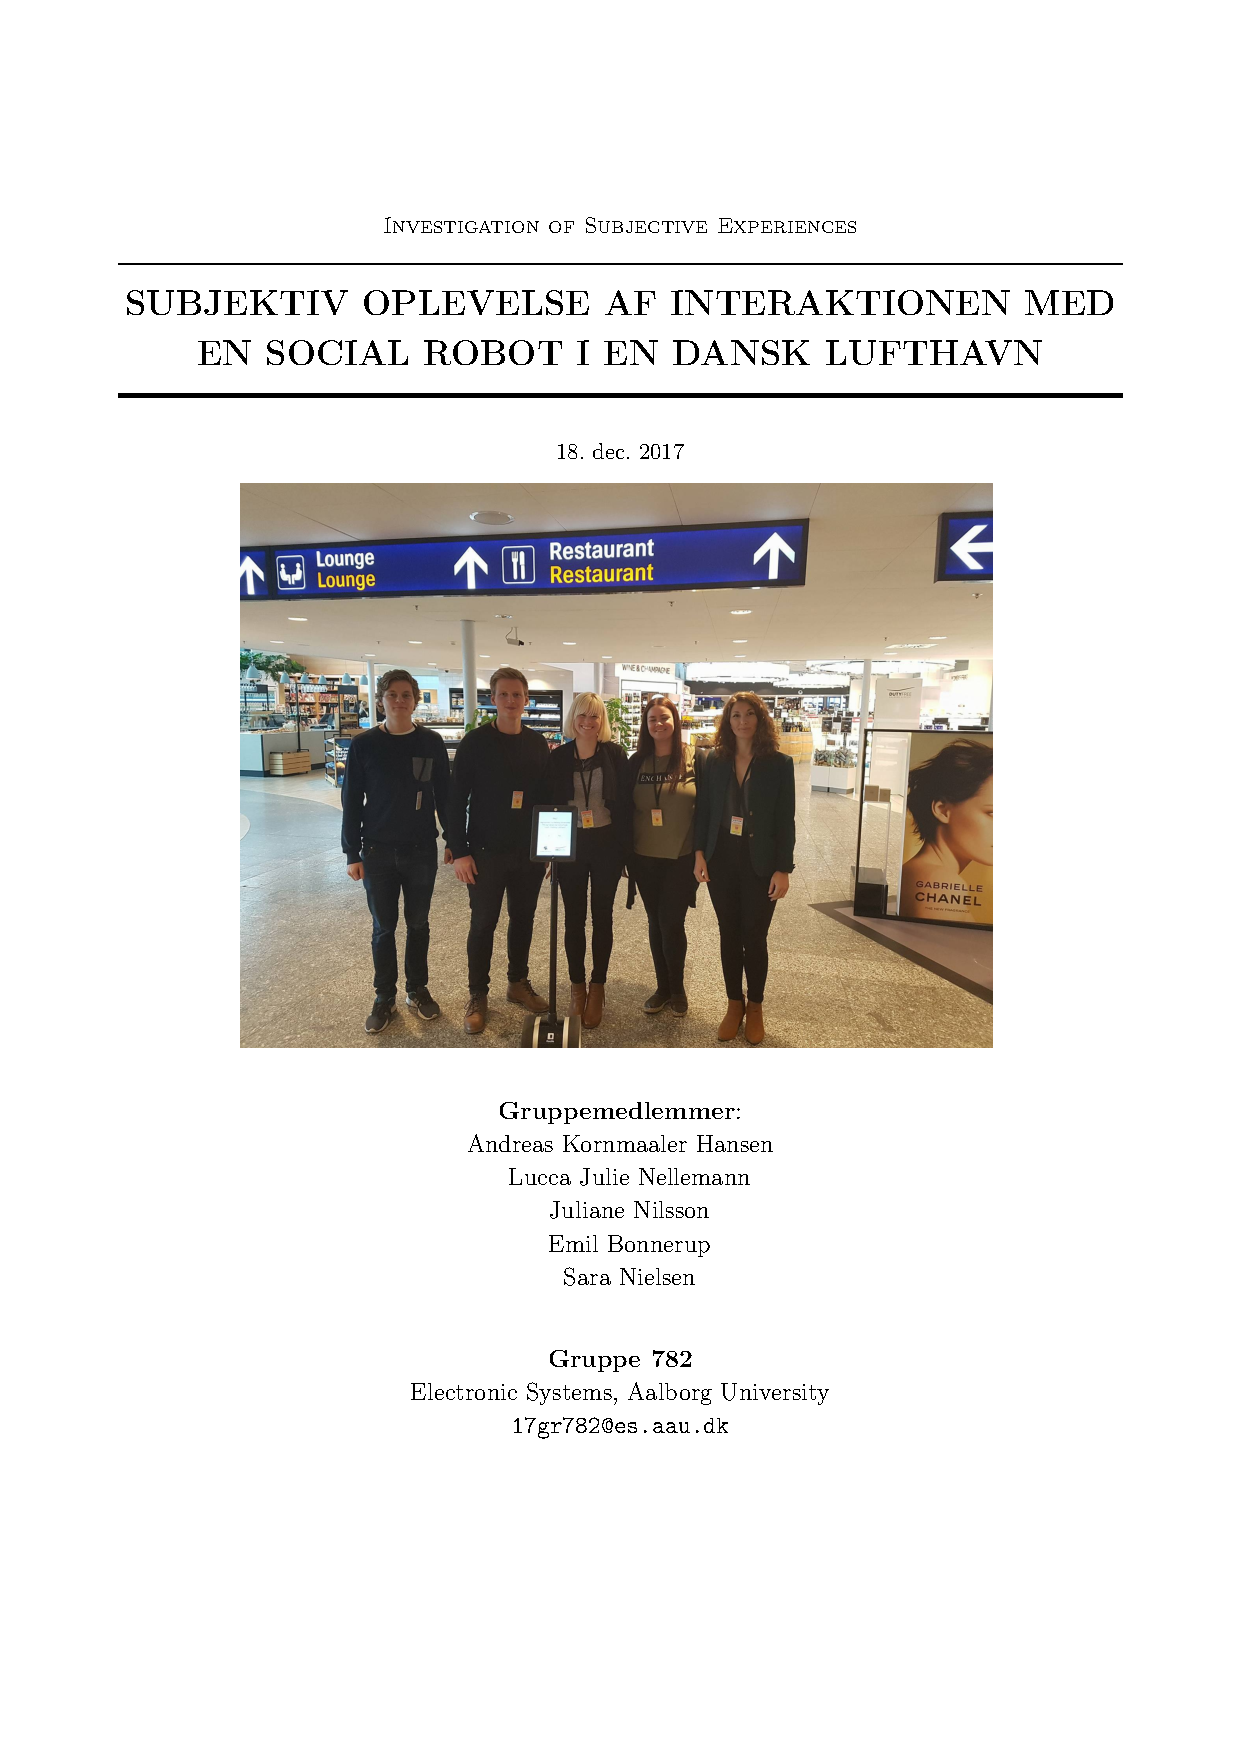
\includepdf{Chapter/Formalia/Forside.pdf}                      %Inkluderer første side af "Forside.PDF"
%\cleardoublepage %Laver en tom side 
%\label{Abstract}
% As a general rule, do not put math, special symbols or citations
% in the abstract
Social robots are expected to play a much bigger role in the near future. This calls for research in determining how these social robots are supposed to behave. This paper presents an ecological field study and investigates the subjective experience of social robots in Aalborg Airport (AAL). Travellers were recruited by a remote controlled robot from Double Robotics, Inc., which had a tablet with an interface asking if it may help them with wayfinding in AAL. When the participants had chosen their location they were asked to follow the robot and led to a semi-structured interview about their first impressions. In total the study includes 30 participants from 8 to 62 years (M=37.9, SD=17.1). The observations and the participants' statements were coded using an Affinity Diagram. 567 affinity notes were sorted and ended up with 10 categories of which the main categories revolved around appearance, behaviour, approach and trust. 


%method
%result
%conclusion

%\cleardoublepage %Laver en tom side 
%% OBS: Many of the commands in this document rely on definitions from another tex-document (Metadata.tex) prior to this one
% Udarbejdet af: Jesper Nørgaard (jesper@noergaard.eu) 10. april 2012


\cleardoublepage
\phantomsection
\pdfbookmark[0]{Titelblad}{Titelblad}
\thispagestyle{empty}

\begin{minipage}[t]{0.48\textwidth}
\vspace*{-25pt}

\includegraphics[height=4cm]{++AAU-Logo++}
\end{minipage}
\hfill
\begin{minipage}[t]{0.48\textwidth}
{\small 
\textbf{v/ Institut for\\
\institutionname}\\
\studyname\\
\adress\\
\city\\
}
\end{minipage}
%
\vspace*{1cm}
%
\begin{minipage}[t]{0.48\textwidth}
\textbf{Titel:} \\[5pt]\bigskip\hspace{2ex}
\projectname\vspace{-2.75ex}\\ \hspace{2ex}

%\textbf{Titel:} \\[5pt]\bigskip\hspace{2ex}
%\projectname\vspace{-2.75ex}\\\bigskip\hspace{2ex}
%\projectnameextension\\
%
\textbf{Projekt:} \\[5pt]\bigskip\hspace{2ex}
\semestername

\textbf{Projektperiode:} \\[5pt]\bigskip\hspace{2ex} \projectperiod

\textbf{Projektgruppe:} \\[5pt]\bigskip\hspace{2ex}
\groupname

%\textbf{Email:} \\[5pt]\bigskip\hspace{2ex}
%\groupemail

\textbf{Vejleder:} \\[5pt]\hspace*{2ex}
\supervisor \\\hspace*{2ex}

%\textbf{Sidetal:} \numberofpages \\ %Antal tekst sider
%\textbf{Antal bilag:} \numberofappendix \\ %Antal bilag
%\textbf{Afsluttet:} \finishdate\ \finishyear
\end{minipage}
%
\begin{minipage}[t]{0.483\textwidth}
\textbf{Synopsis:} \\[5pt]
\fbox{\parbox{7cm}{\bigskip%\fxwrite{Synopsis}
I dette studie undersøges danske rejsendes subjektive oplevelse af at blive betjent af en social robot i Aalborg Lufthavn (AAL), gennem to økologiske feltstudier. I begge tests blev de rejsende tilnærmet af en Double robot, som tilbød at hjælpe dem med at finde vej. Efter en kort interaktion, beder robotten den rejsende følge efter sig mod den valgte destination. I første test kørte robotten de rejsende hen til et semi-struktureret interview om deres oplevelse. På baggrund af observationer og interviews fra denne test, blev 567 affinity notes kategoriseret i et affinity diagram med 10 kategorier, hvorfra vigtige parametre i forhold til brugeroplevelsen af sociale robotter udledes. På baggrund af disse parametre udvikles 24 skalaer, som efterfølgende er blevet anvendt i lufthavnen. I anden test ledte robotten de rejsende hen til en forsøgsleder, hvor de på de udviklede skalaer vurderede deres oplevelse af interaktionn med robotten. Resultaterne fra anden test blev analyseret med Principal Component Analysis, som viste både positive og negative korrelationer mellem flere af skalaerne.\bigskip}}
\end{minipage}

\vspace{-5 mm} % Sætter afstand fra ovenstående. Skal op eller nedjusteres, så det ser pænt ud og holder sig på én side.
\noindent
\textbf{Deltagere:}

\vspace{5 mm} % Sætter afstand fra ovenstående. (Afstanden mellem Overskriften "Deltagere" og underskriftslinjerne)

\begin{table}[H]
	\centering
		\begin{tabular}{c c c}
			\underline{\phantom{mmmmmmmmmmmmmmmmmmm}} & 	\underline{\phantom{mmmmmmmmmmmmmmmmmmm}} \\
			\groupmemberI & \groupmemberII \\
		\end{tabular}
\end{table}
\begin{table}[H]
	\centering
		\begin{tabular}{c c c}
			\underline{\phantom{mmmmmmmmmmmmmmmmmmm}} & 	\underline{\phantom{mmmmmmmmmmmmmmmmmmm}} \\
			\groupmemberIII & \groupmemberIIII \\
		\end{tabular}
\end{table}
\begin{table}[H]
	\centering
		\begin{tabular}{c c c}
			\underline{\phantom{mmmmmmmmmmmmmmmmmmm}}\\
			\groupmemberIIIII \\
		\end{tabular}
\end{table}
\vfill

%{\footnotesize\itshape Rapportens indhold er frit tilgængeligt, men offentliggørelse (med kildeangivelse) må kun ske efter aftale med forfatterne.}

%{\footnotesize\itshape The content of the report is freely available, but publication (with source reference) may only take place in agreement with the authors.}
\cleardoublepage

%\cleardoublepage
%\chapter*{Forord}
\label{Forord}
Denne rapport er udarbejdet af \groupname; \groupmembers\ i perioden \projectperiod. Gruppen er 7. Semesterstuderende fra studiet \studyname\ på \universityname\ og har haft \supervisor\ som vejleder. Gruppen retter en stor tak til vejleder \supervisor\ for god vejledning. Ydermere rettes en stor tak til Karl Damkjær Hansen for...SKRIV
%
\section*{Læsevejledning}
\label{Laesevejledning}
Arbejdsbladene er skrevet kronologisk, efterhånden som projektet er skredet frem. De kan med fordel læses kronologisk, da nogle afsnit antager, at læseren har kendskab til tidligere afsnit i arbejdsbladene. Der vil dog også være henvisninger til tidligere omtalte emner, når relevant.

\subsection*{Henvisninger}
Alle henvisninger i rapporten fungerer som hyperlinks, som illustreret i eksemplet her: \autoref{fig:CategorizationOfRobots}.
%
\subsection*{Kildehenvisninger}
Kildehenvisninger angives enten som en del af teksten eller i parentes. Et eksempel på de to kildehenvisningsmetoder: \textcite[s. 13]{PDF:RobotShiftFromIPtoSR} eller \parencite[s. 13]{PDF:RobotShiftFromIPtoSR}. Såfremt der refereres til en bestemt del af kilden, angives dette med sidetal, eksempelvis; s. 13 for én bestemt side eller ss. 1-3 for flere sider.
%
\subsection*{Afsnitshenvisning}
Afsnitshenvisninger angives med et afsnitsnummer efterfulgt af et afsnitsnavn. Et eksempel på en afsnitshenvisning: \fullref{KarakteriseringAfSocialRobot}. Samme gør sig gældende for kapitler.
%
\subsection*{Figurhenvisning}
Henvisninger til figurer angives med et decimaltal, som først gengiver kapitlets nummer efterfulgt af figurnummeret i det pågældende kapitel. Et eksempel på en figurhenvisning: \autoref{fig:CategorizationOfRobots}, der svarer til figur 1 i kapitel 2. 
%
\subsection*{Henvisninger til elektronisk bilag}
Henvisninger til det elektroniske bilag angives med en afsnitshenvisning, hvor stien til det pågældende bilag fremgår i det pågældende afsnit. 

\subsection*{Decimalseparator}
Der benyttes "." (punktum), som decimalseparator. %Inkluder forord
%\cleardoublepage

                              
\tableofcontents* %Indholdsfortegningelse * = uden sidetal

\mainmatter	%Starter med at nummere siderne

\chapter*{Pitch perception - JND}
%
The purpose of this study is to evaluate the differential threshold, known as Just Noticeable Difference (JND), of pitch perception. Webers law states that the smallest detectable change in perception, \textit{$\Delta$I}, is equal to a constant, \textit{k}, times the physical stimulus intensity, \textit{I}. 
%
\begin{equation}
\Delta I = k \cdot I
\end{equation}
%
The constant, \textit{k}, is known as the Weber Fraction for a particular sensory dimension.
%

\section*{Methods}
%
The psychometric method used for stimuli presentation is the Method of Constant Stimuli which prescribe that the experimenter chooses a number of stimulus intensities and a reference intensity. In this study the stimulus intensity refers to frequency and the test subject reports which of the two stimuli are highest in pitch. The response is presented as a psychometric function. 

The chosen frequencies have to be a qualified guess about where the test subjects differential threshold is. In our study we base the qualified guess on the differential threshold found by \citet{Wier1977} at 800 Hz which is approximately 1.2 Hz. It is important that the intensity range covers intensities above and below the actual differential threshold so there must be stimuli which the test subject always report the correct answer to and vice versa. Based on a pilot test the intensity range was expanded with higher frequency differences because some of the test subjects did not reach a plateau of 100 \% correct answers. Based on the differential threshold approximation from \citet{Wier1977} and the pilot test, the intensity range consists of frequencies with a logarithmic difference from 800 Hz starting from 0.15 Hz to 76.8 Hz. Each frequency is repeated 10 times which leads to a total of 100 trials per test subject.  

Data collections is done by Two-Alternative Forced Choice (2-AFC). A more objective measure is obtained with 2-AFC because the test subjects are forced to make an answer whether or not they actually heard a difference between the two stimuli \citep[p. 1219]{Ehrenstein1999}. 2-AFC accounts for criterium biases when using multiple test subjects who might have different response criteria when answering which of the two frequency had the highest pitch. Criterium biases are avoided because the test subjects are forced to answer,  whether or not they have perceived a difference. When using this method there is a 50 \% chance of guessing which of the two stimuli had the highest pitch and therefore the JND is found where 75 \% of the answers are correct.\\[5mm]
%
In contrast to the two other classical psychometric methods the Method of Constant Stimuli prescribes randomization of stimuli representation which eliminates anticipation and habituation \citep[p. 15]{Poulsen2005}. One disadvantage with Method of Constant Stimuli is the measurement time. Each added repetition or stimulus intensity will add extra time in which the subjects must focus on pitch differences. This prolonged measurement time might lead to fatigue and risk of an altered differential threshold \citep[p. 16]{Poulsen2005}. 
%

\subsection*{Experimental setup}
%
The equipment used for the study is a pair of Bang $\&$ Olufsen H6 headphones, a Lenovo Thinkpad with a fixed 10 \% volume, and a programme (TwoAFC\_pitch) running in MatLab for stimuli presentation. The two tones are presented as A and B on the screen and the test subject has to choose the one they perceive as having the highest pitch by pressing one of the buttons accordingly. The experiment was conducted in a group room located on the 1st floor of Fredrik Bajers vej 7B, B2-207. \autoref{fig:experiment} illustrates the experimental setup.
%
\begin{figure}[H]
\centering
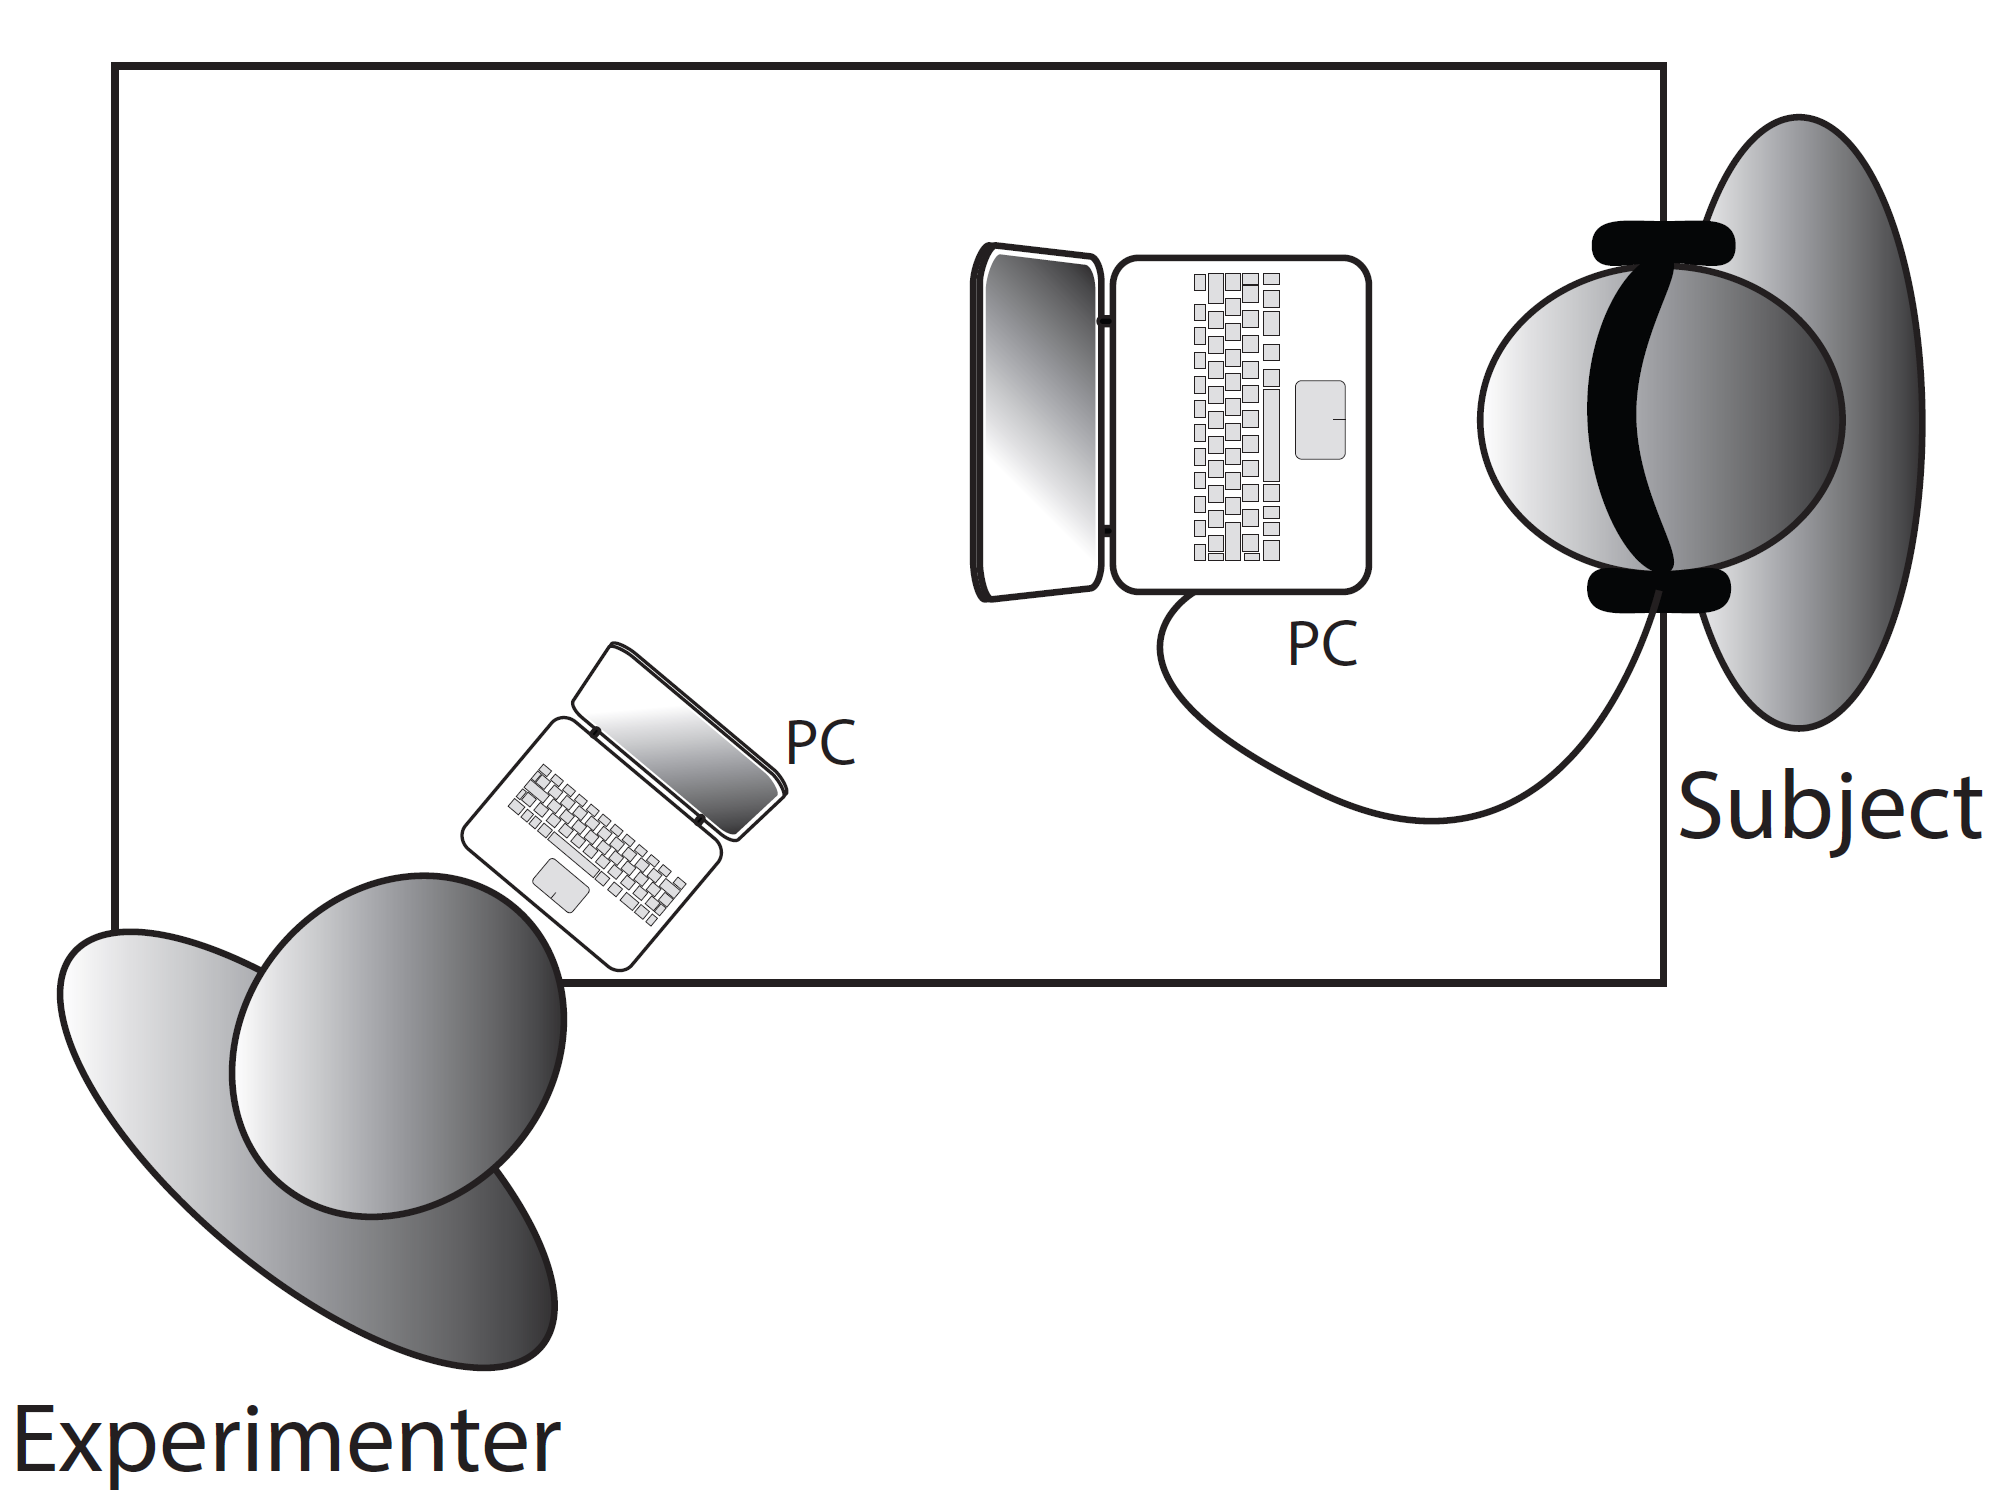
\includegraphics[width = 0.5\textwidth]{Figure/Vores_Figurer/experiment.png} 
\caption{A sketch of the experimental setup}
\label{fig:experiment}
\end{figure}
%

\subsection*{Test subjects}
%
Five test subjects were used in the test including two males and three females in the age of 23 to 24 (mean = 23.4). All of which are Engineering Psychology students at Aalborg University.

\subsection*{Pilot test}
%
Based on a pilot test it is decided to expand the stimuli intensity range down to 0.15 Hz and up to 76.8 Hz from the original range of intensities 0.3 Hz, 0.6 Hz, 1.2 Hz, 2.4 Hz, 4.8 Hz, 9.6 Hz. This is done because the female test subjects had problems detecting any difference in pitch even at the highest frequency differences.

\section*{Results}
%
On \autoref{fig:AllSubjects} data from each test subject is presented along with the psychometric function. The response from the subjects are represented as the percentage of correct answers to each frequency difference, $\Delta$f.
% 
\begin{figure}[H]
\centering
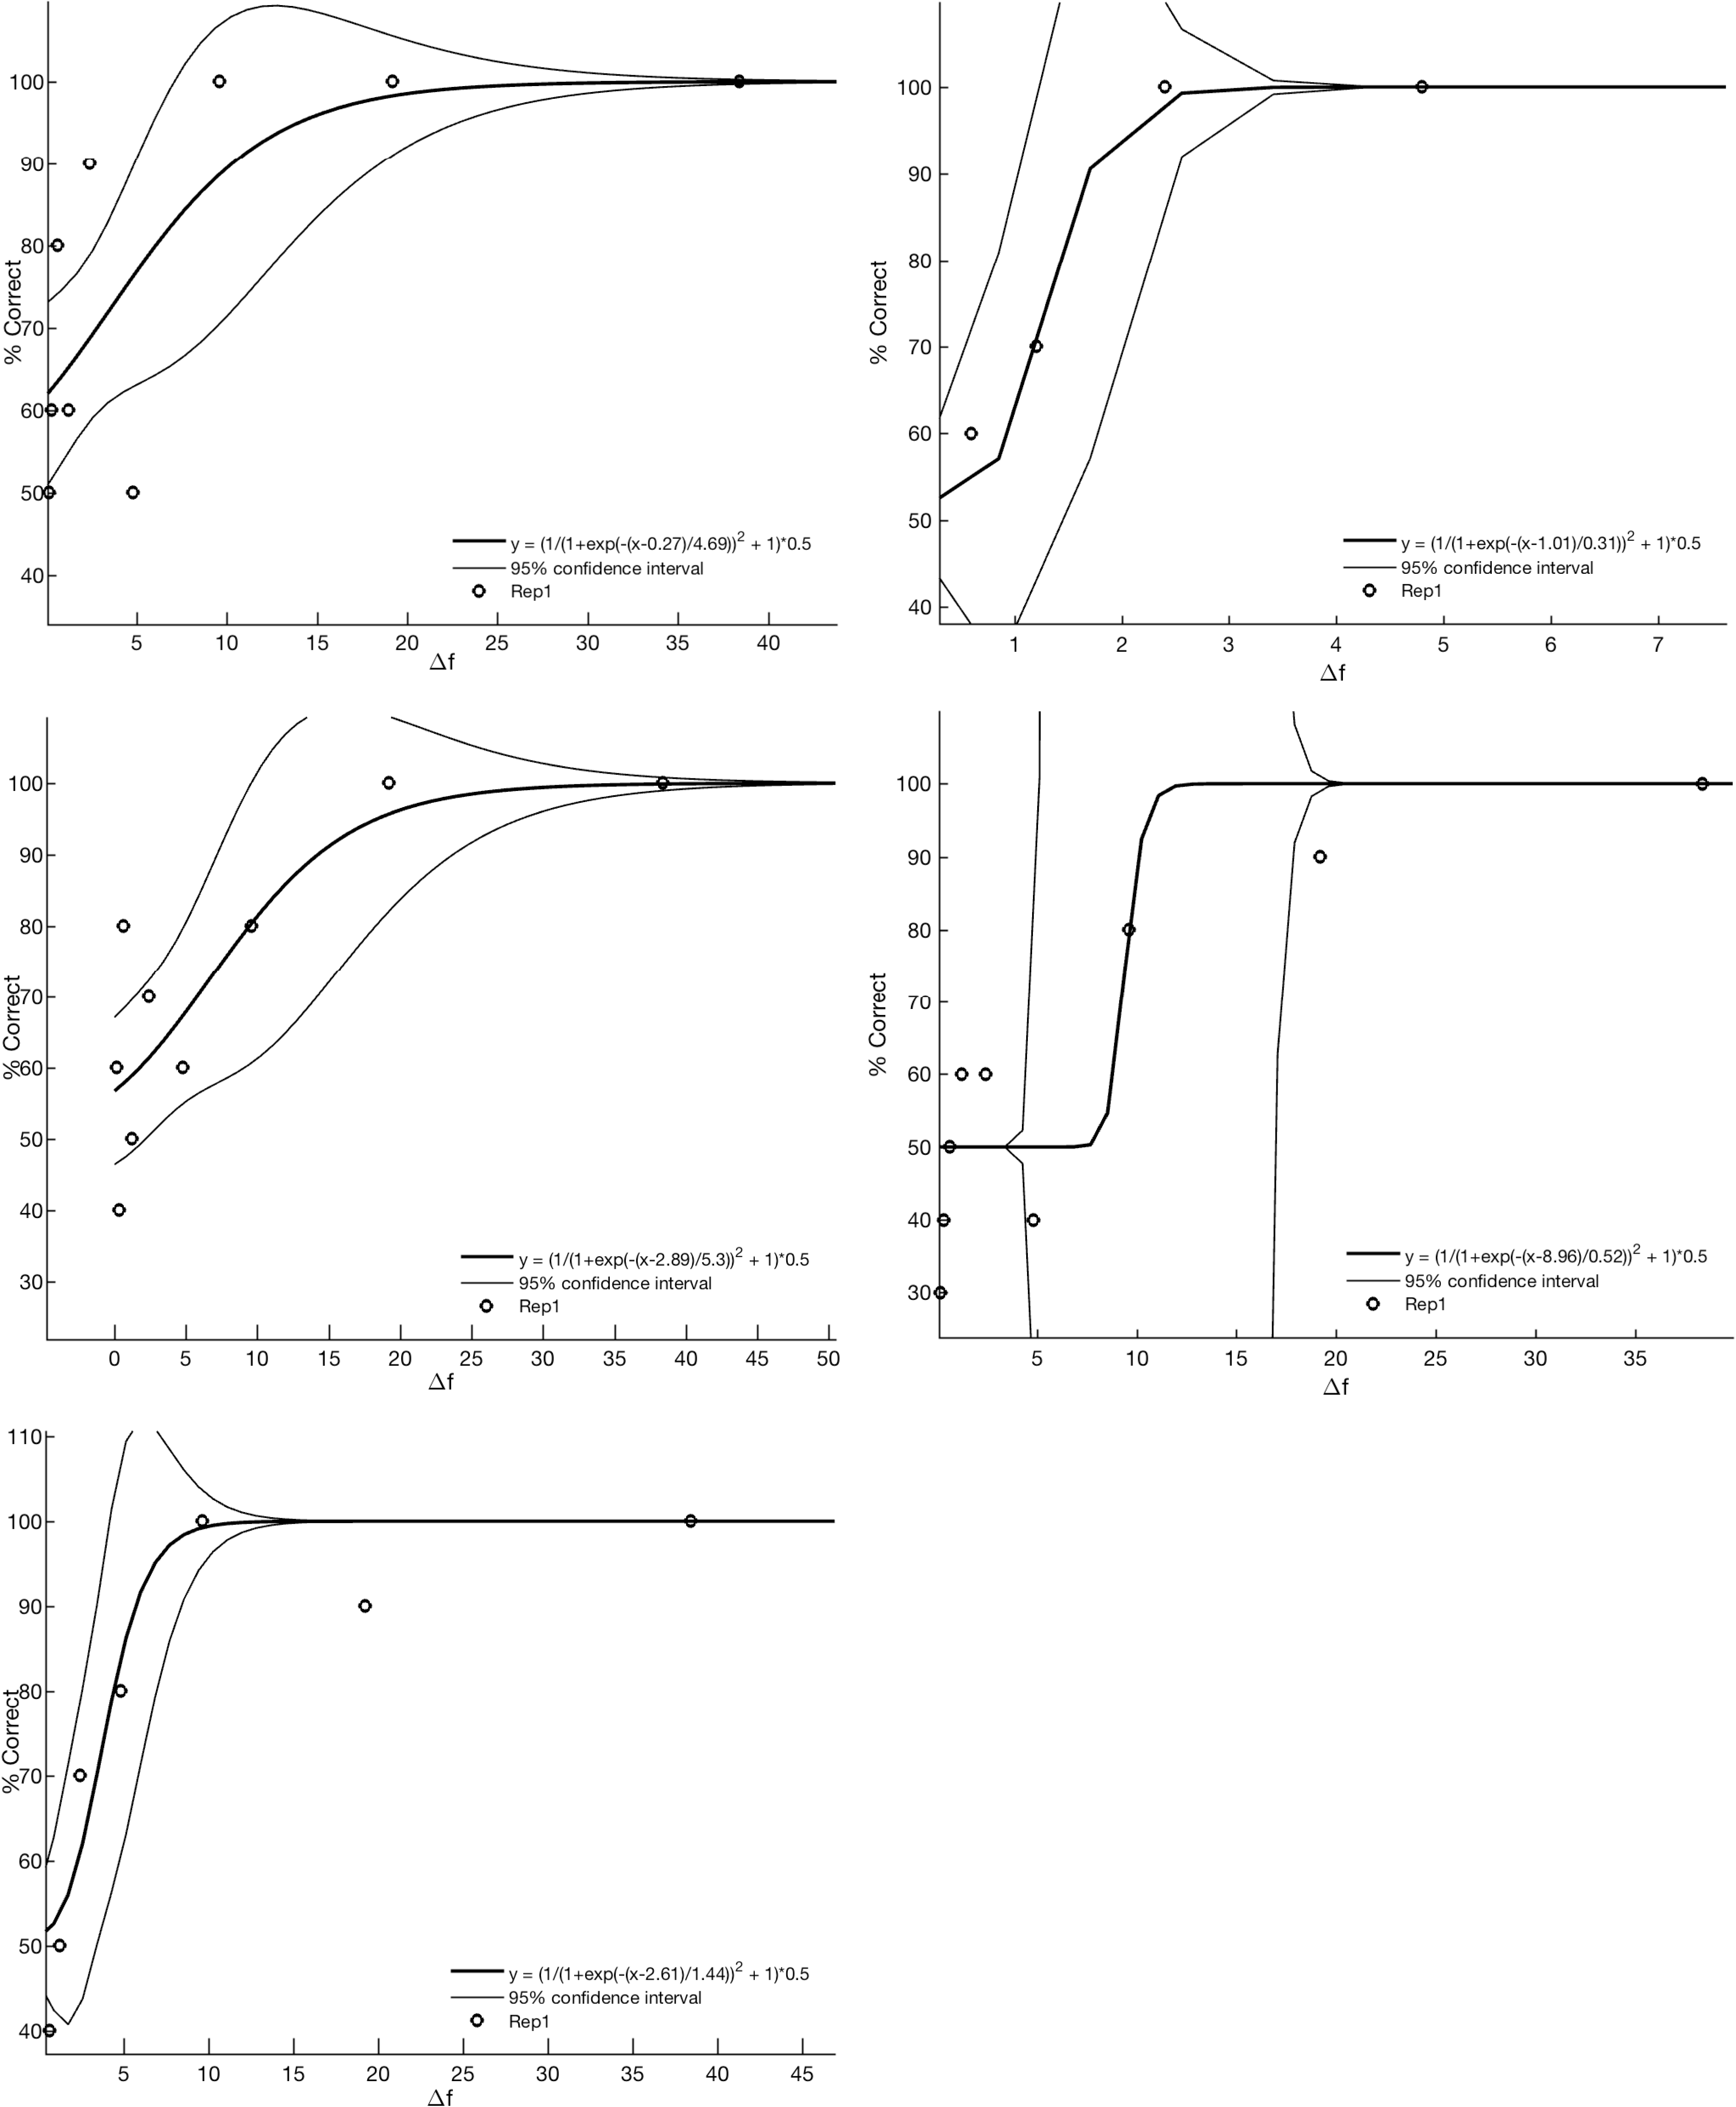
\includegraphics[width = \textwidth]{Figure/Vores_Figurer/AllSubjects.png} 
\caption{Raw data and fitted psychometric function for all five subjects.}
\label{fig:AllSubjects}
\end{figure}
%
\section*{Analysis}
%
A 2-AFC method is used to collect data which leaves a 50 \% chance of guessing the right answer of the two possibilities. The point for JND is therefore at 75 \%.

From the fitted psychometric function for each subject the JND is read at 75 \% correct answered. In \autoref{tab:JND} the individual test subjects JND are presented along with a calculated mean JND which is 5.31 Hz. 
%
\begin{table}[H]
\centering
\begin{tabular}{l|c}
Subject     & JND ($\Delta$f at 75\%) \\\hline
Subject 1   & 4.40 Hz                 \\\hline
Subject 2   & 1.28 Hz                 \\\hline
Subject 3   & 7.56 Hz                 \\\hline
Subject 4   & 9.42 Hz                 \\\hline
Subject 5   & 3.88 Hz                 \\\hline
mean JND & 5.31 Hz       
\end{tabular}
\caption{JND for all test subjects and mean JND.}
\label{tab:JND}         
\end{table}
\noindent
%
From Webers law the Weber fraction, \textit{k}, can be calculated. According to this sample, the smallest detectable change in pitch perception, \textit{$\Delta$I}, is the mean JND at 5.31 Hz, when compared to the physical stimulus intensity, \textit{I}, of 800 Hz.
% 
\begin{equation}
5.31 Hz = k \cdot 800 Hz \Rightarrow k = \frac{5.31 Hz}{800 Hz} = 0.007
\end{equation}
%
This Weber fraction allows for calculating differential threshold at other intensities, \textit{I}. 
%

\section*{Discussion and conclusion}
%
In the pilot test the female test subjects had problems detecting differences in pitch, especially when the difference between the two frequencies was small, while the male subjects did not experience these problems. This might be due to the fact that one of the male test subjects have more expertise in listening to music and its specific characteristics e.g. when tuning a guitar. Furthermore the subjects might not answer based on the same criterions e.g. they might have different understandings of the word “pitch”. When trying to agree upon a common definition of “pitch”, there might also be different understandings of the words used to describe it.  

From the pilot test it became clear that some of the test subject’s differential threshold was outside the range of the chosen stimuli intensities. Therefore it was decided to expand the intensity range with more frequencies so every test subjects differential threshold would be included. If a test with more subjects had been done, it would likewise have been important to use a frequency range which includes every subject’s differential threshold. Furthermore, a study with more test subjects could be more representative for the true JND.\\[5mm] 
%
Problems with the experimental design could be that the test subjects listens to the tones right after each other. This could be an issue because the subjects easily can compare the first tone of a trial with the last tone of the previously trial, which can influence their responses because they base their answer on memory. Other problems could be the way subjects pressed the A and B button on the computer screen. Some of the subjects used the touch function on the screen while others used the mousepad. For the subjects using the mousepad the mouse on the screen did not move from the chosen button after every comparison and therefore the test subject could be biased to choose the previously pressed button. This issue could have been solved if the subjects after each trial pressed a separate “next” button which will force the subjects to move the cursor to a different position.\\[5mm]
%  
The results shows that the mean JND at 75 \% is 5.31 Hz, which is a bit higher than the expected 1.2 Hz. This might be due to variables affecting the outcome of this study, including ambient noise, distractions and fatigue. If the test was done in an sound isolated lab JND might have been closer to the approximately 1.2 Hz from \citet{Wier1977} findings. Furthermore, \citet{Wier1977} might have used different levels of pitch and more repetitions, which can contribute to different results.\\[5mm] 
%
The calculated Weber fraction should allow for calculating differential threshold at other intensities, \textit{I}. When doing this it is important to be aware of the conditions in which the Weber fraction is calculated. 





 


\cleardoublepage


%%% Kilder %%%%
\nocite{Holmqvist2015}
\begingroup
	\raggedright
	\bibliography{Bib/Bibliography}			                    % Litteraturlisten inkluderes
\endgroup


%%%% Appendiks %%%%
%\appendix
%\appendixpage*
%\input{Chapter/Appendiks/Appendiks}
\end{document}
